% This file was created by tikzplotlib v0.9.8.
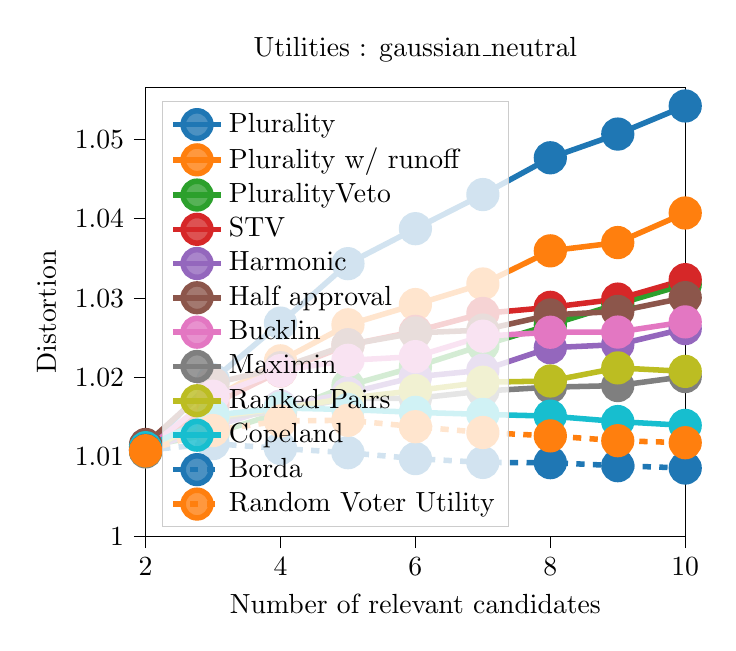
\begin{tikzpicture}

\definecolor{color0}{rgb}{0.12156862745098,0.466666666666667,0.705882352941177}
\definecolor{color1}{rgb}{1,0.498039215686275,0.0549019607843137}
\definecolor{color2}{rgb}{0.172549019607843,0.627450980392157,0.172549019607843}
\definecolor{color3}{rgb}{0.83921568627451,0.152941176470588,0.156862745098039}
\definecolor{color4}{rgb}{0.580392156862745,0.403921568627451,0.741176470588235}
\definecolor{color5}{rgb}{0.549019607843137,0.337254901960784,0.294117647058824}
\definecolor{color6}{rgb}{0.890196078431372,0.466666666666667,0.76078431372549}
\definecolor{color7}{rgb}{0.737254901960784,0.741176470588235,0.133333333333333}
\definecolor{color8}{rgb}{0.0901960784313725,0.745098039215686,0.811764705882353}

\begin{axis}[
legend cell align={left},
legend style={
  fill opacity=0.8,
  draw opacity=1,
  text opacity=1,
  at={(0.03,0.97)},
  anchor=north west,
  draw=white!80!black
},
tick align=outside,
tick pos=left,
title={Utilities : gaussian\_neutral},
x grid style={white!69.0196078431373!black},
xlabel={Number of relevant candidates},
xmin=2, xmax=10,
xtick style={color=black},
y grid style={white!69.0196078431373!black},
ylabel={Distortion},
ymin=1, ymax=1.05648827913636,
ytick style={color=black}
]
\addplot [line width=2pt, color0, mark=*, mark size=5, mark options={solid}]
table {%
2 1.01096263476543
3 1.01970339880206
4 1.02684977529115
5 1.03433946383179
6 1.03874545942846
7 1.04304520346914
8 1.04767966304752
9 1.05066757868412
10 1.05420730465504
};
\addlegendentry{Plurality}
\addplot [line width=2pt, color1, mark=*, mark size=5, mark options={solid}]
table {%
2 1.01089939474617
3 1.01736212318756
4 1.02209579199946
5 1.02663821212555
6 1.02918602816582
7 1.03177901635207
8 1.03595384292573
9 1.03699832820833
10 1.04072481690105
};
\addlegendentry{Plurality w/ runoff}
\addplot [line width=2pt, color2, mark=*, mark size=5, mark options={solid}]
table {%
2 1.01133119750919
3 1.01291562334206
4 1.01558309310413
5 1.01896746889164
6 1.02134381807571
7 1.0240559861307
8 1.02662575062555
9 1.02924899165495
10 1.03171675626086
};
\addlegendentry{PluralityVeto}
\addplot [line width=2pt, color3, mark=*, mark size=5, mark options={solid}]
table {%
2 1.01097470624416
3 1.0166393664422
4 1.02079745592151
5 1.02408271413775
6 1.02581093240879
7 1.02806583575764
8 1.02883852077921
9 1.02987560892378
10 1.03232488734146
};
\addlegendentry{STV}
\addplot [line width=2pt, color4, mark=*, mark size=5, mark options={solid}]
table {%
2 1.01085724029089
3 1.01380623032459
4 1.01640469517179
5 1.01800845256855
6 1.02007371083227
7 1.02091932449965
8 1.02375125013161
9 1.02414090920821
10 1.02615952855934
};
\addlegendentry{Harmonic}
\addplot [line width=2pt, color5, mark=*, mark size=5, mark options={solid}]
table {%
2 1.01155848003403
3 1.01924551929304
4 1.02122739945216
5 1.02411776987945
6 1.02560997436633
7 1.02597335956032
8 1.02787888740664
9 1.02832450850003
10 1.03006051928308
};
\addlegendentry{Half approval}
\addplot [line width=2pt, color6, mark=*, mark size=5, mark options={solid}]
table {%
2 1.01088169013085
3 1.01763983624109
4 1.02086287425694
5 1.02216181298533
6 1.02262331473008
7 1.02520003234868
8 1.02569799001282
9 1.02572067249486
10 1.02700267919232
};
\addlegendentry{Bucklin}
\addplot [line width=2pt, white!49.8039215686275!black, mark=*, mark size=5, mark options={solid}]
table {%
2 1.01061946244897
3 1.01484996088822
4 1.01572316574784
5 1.01737996115891
6 1.01736351127246
7 1.01828979585341
8 1.0187741019758
9 1.01898087289392
10 1.02011938835578
};
\addlegendentry{Maximin}
\addplot [line width=2pt, color7, mark=*, mark size=5, mark options={solid}]
table {%
2 1.01076469889298
3 1.01502588656443
4 1.01610959610224
5 1.01738609404913
6 1.01834767911112
7 1.01939609488234
8 1.01955790270213
9 1.02120604446635
10 1.02076624257044
};
\addlegendentry{Ranked Pairs}
\addplot [line width=2pt, color8, mark=*, mark size=5, mark options={solid}]
table {%
2 1.01115493301185
3 1.01525076015977
4 1.01615272702117
5 1.01595991159512
6 1.01560653581625
7 1.01534738640733
8 1.01513027558545
9 1.01444400028152
10 1.01396066959295
};
\addlegendentry{Copeland}
\addplot [line width=2pt, color0, dashed, mark=*, mark size=5, mark options={solid}]
table {%
2 1.01082796355864
3 1.01166348632712
4 1.01105412504367
5 1.01052142891205
6 1.00977681806624
7 1.00929689287106
8 1.00926433786765
9 1.0088827128464
10 1.00858781502864
};
\addlegendentry{Borda}
\addplot [line width=2pt, color1, dashed, mark=*, mark size=5, mark options={solid}]
table {%
2 1.01076996860175
3 1.01331584665326
4 1.01452557399971
5 1.01460333457308
6 1.01379681202178
7 1.01306416408095
8 1.01263925445096
9 1.01203313246624
10 1.01177931503543
};
\addlegendentry{Random Voter Utility}
\end{axis}

\end{tikzpicture}
